\documentclass[11pt]{article}

\usepackage[margin=1in]{geometry}
\usepackage{amsfonts, amsmath, amssymb}
\usepackage{fancyhdr, float, graphicx}
\usepackage[utf8]{inputenc} % Required for inputting international characters
\usepackage[T1]{fontenc} % Output font encoding for international characters
\usepackage{fouriernc} % Use the New Century Schoolbook font
\usepackage[nottoc, notlot, notlof]{tocbibind}
\usepackage{listings}
\usepackage{xcolor}
\usepackage{blindtext}
\usepackage{hyperref}
\hypersetup{
	colorlinks=true,
	linkcolor=black,
	filecolor=magenta,
	urlcolor=blue,
	pdfpagemode=FullScreen,
}

\definecolor{codegreen}{rgb}{0,0.6,0}
\definecolor{codegray}{rgb}{0.5,0.5,0.5}
\definecolor{codepurple}{rgb}{0.58,0,0.82}
\definecolor{backcolour}{rgb}{0.95,0.95,0.92}

\lstdefinestyle{mystyle}{
	backgroundcolor=\color{backcolour},
	commentstyle=\color{codegreen},
	keywordstyle=\color{magenta},
	numberstyle=\tiny\color{codegray},
	stringstyle=\color{codepurple},
	basicstyle=\ttfamily\footnotesize,
	breakatwhitespace=false,
	breaklines=true,
	captionpos=b,
	keepspaces=true,
	numbers=left,
	numbersep=5pt,
	showspaces=false,
	showstringspaces=false,
	showtabs=false,
	tabsize=2
}

\lstset{style=mystyle}

% Header and Footer
\pagestyle{fancy}
\fancyhead{}
\fancyfoot{}
\fancyhead[L]{\textit{\Large{Attack Reserach and Documentation - Fourth Year B. Tech}}}
\fancyhead[R]{\textit{Krishnaraj T}}
\fancyfoot[C]{\thepage}
\renewcommand{\footrulewidth}{1pt}

\begin{document}

\begin{titlepage}
	\centering

	%---------------------------NAMES-------------------------------

	\huge\textsc{
		MIT World Peace University
	}\\

	\vspace{0.75\baselineskip} % space after Uni Name

	\LARGE{
		Attack Research and Documentation\\
		Fourth Year B. Tech, Semester 8
	}

	\vfill % space after Sub Name

	%--------------------------TITLE-------------------------------

	\rule{\textwidth}{1.6pt}\vspace*{-\baselineskip}\vspace*{2pt}
	\rule{\textwidth}{0.6pt}
	\vspace{0.75\baselineskip} % Whitespace above the title

	\huge{\textsc{
        Hands on Exercise on Preserving Digital Evidence for Legal purposes
    }} \\

	\vspace{0.5\baselineskip} % Whitespace below the title
	\rule{\textwidth}{0.6pt}\vspace*{-\baselineskip}\vspace*{2.8pt}
	\rule{\textwidth}{1.6pt}

	\vspace{1\baselineskip} % Whitespace after the title block

	%--------------------------SUBTITLE --------------------------	

	\LARGE\textsc{
		Lab Assignment 6
	} % Subtitle or further description
	\vfill

	%--------------------------AUTHOR-------------------------------

	Prepared By \vspace{0.5\baselineskip} % Whitespace before the editors

	\Large{
		Krishnaraj Thadesar \\
		Cyber Security and Forensics\\
        Batch A1, PA 15
	}

	\vspace{0.5\baselineskip} % Whitespace below the editor list
	\today

\end{titlepage}

\tableofcontents
\thispagestyle{empty}
\clearpage

\setcounter{page}{1}

\section{Introduction}
\begin{itemize}
    \item This report documents the use of two digital forensics tools --- \textbf{FTK Imager Lite} and \textbf{Autopsy}.
    \item The aim is to simulate data deletion scenarios and analyze the ability to recover data.
    \item Screenshots are attached as visual evidence for each step.
\end{itemize}

\section{Tools Used}

\subsection{FTK Imager Lite}
FTK Imager Lite is a lightweight, freeware imaging tool developed by Exterro. It is widely used in digital forensics for creating forensic images of storage devices. The tool is designed to ensure data integrity and is capable of generating MD5 and SHA1 hash values for verification. Key features of FTK Imager Lite include:
\begin{itemize}
    \item \textbf{Forensic Imaging:} Allows users to create bit-by-bit copies of storage devices, ensuring no data is altered during the process.
    \item \textbf{Hash Verification:} Generates hash values (MD5 and SHA1) to confirm the integrity of the forensic image.
    \item \textbf{Preview Functionality:} Enables users to preview files and folders on the storage device before imaging.
    \item \textbf{Support for Multiple Formats:} Supports imaging in various formats, including E01, DD, and raw image formats.
    \item \textbf{Logical and Physical Imaging:} Provides options to create logical images (specific files or folders) or physical images (entire storage devices).
\end{itemize}
FTK Imager Lite is an essential tool for forensic investigators, ensuring that evidence is preserved in a reliable and verifiable manner.

\subsection{Autopsy}
Autopsy is an open-source, graphical digital forensics platform designed for analyzing disk images and recovering data. It is built on top of The Sleuth Kit (TSK) and provides an intuitive interface for investigators. Key functionalities of Autopsy include:
\begin{itemize}
    \item \textbf{File System Analysis:} Supports analysis of various file systems, including NTFS, FAT, exFAT, and EXT.
    \item \textbf{Deleted File Recovery:} Attempts to recover deleted files and directories from disk images.
    \item \textbf{Keyword Search:} Allows users to search for specific keywords within files and metadata.
    \item \textbf{Timeline Analysis:} Generates a timeline of file activities, helping investigators understand the sequence of events.
    \item \textbf{Artifact Extraction:} Extracts artifacts such as browser history, email data, and registry information.
    \item \textbf{Hash Set Matching:} Compares file hashes against known hash sets to identify suspicious or known files.
    \item \textbf{Modular Architecture:} Supports plugins and modules for extending functionality, such as analyzing mobile devices or network traffic.
\end{itemize}
Autopsy is a powerful tool for forensic analysis, enabling investigators to uncover critical evidence and reconstruct events effectively.

\section{Environment Setup}

\subsection{Installation of FTK Imager Lite}
\begin{itemize}
    \item FTK Imager Lite was downloaded from the official Exterro website.
    \item Terms and conditions were reviewed before installation.
\end{itemize}
\begin{figure}[H]
    \centering
    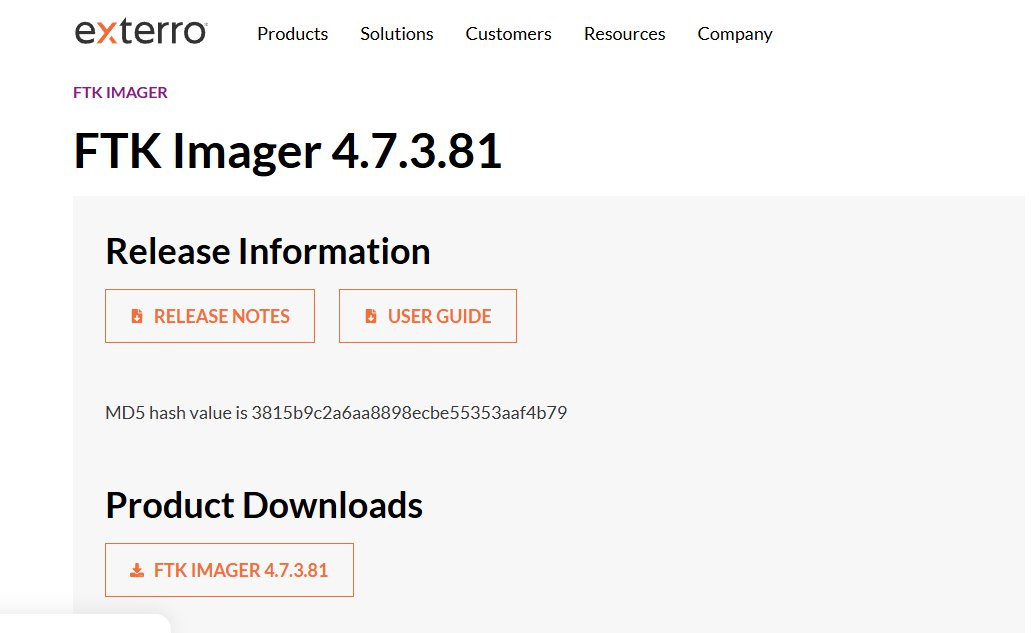
\includegraphics[width=0.99\textwidth]{ftk.jpg}
    \caption{Downloading FTK Imager}
    \label{fig:1}
\end{figure}

\subsection{Installation of Autopsy}
\begin{itemize}
    \item Autopsy was downloaded from \href{https://www.autopsy.com}{https://www.autopsy.com}.
    \item The tool was installed and verified for functionality.
\end{itemize}
\begin{figure}[H]
    \centering
    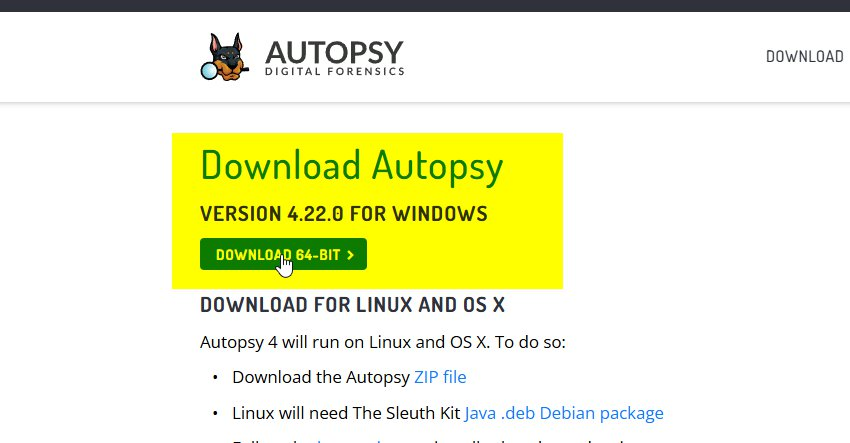
\includegraphics[width=0.99\textwidth]{autopsy.jpg}
    \caption{Downloading Autopsy}
    \label{fig:1}
\end{figure}

\section{Creating Logical Partition and Files}

\subsection{Partition Creation}
\begin{itemize}
    \item A 20MB logical partition was created using the built-in disk management utility.
\end{itemize}
\begin{figure}[H]
    \centering
    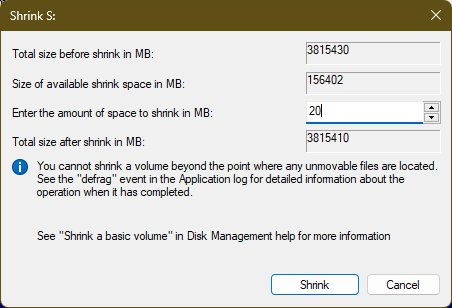
\includegraphics[width=0.8\textwidth]{shrink.jpg}
    \caption{Shrinking Volume to then create a new one. }
    \label{fig:1}
\end{figure}

\subsection{File Creation and Deletion}

\subsubsection{Images}
\begin{itemize}
    \item Multiple files were created in the partition.
    \item A few files were then deleted to simulate data loss.
\end{itemize}
\begin{figure}[H]
    \centering
    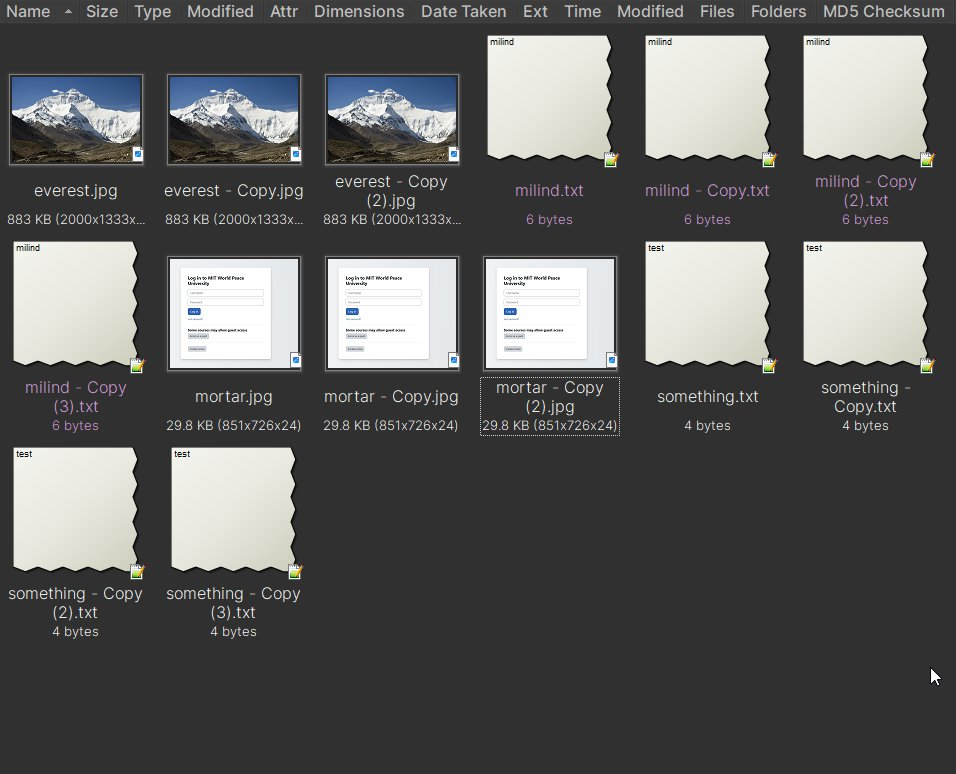
\includegraphics[width=0.99\textwidth]{folder.jpg}
    \caption{Screenshot}
    \label{fig:1}
\end{figure}
\begin{figure}[H]
    \centering
    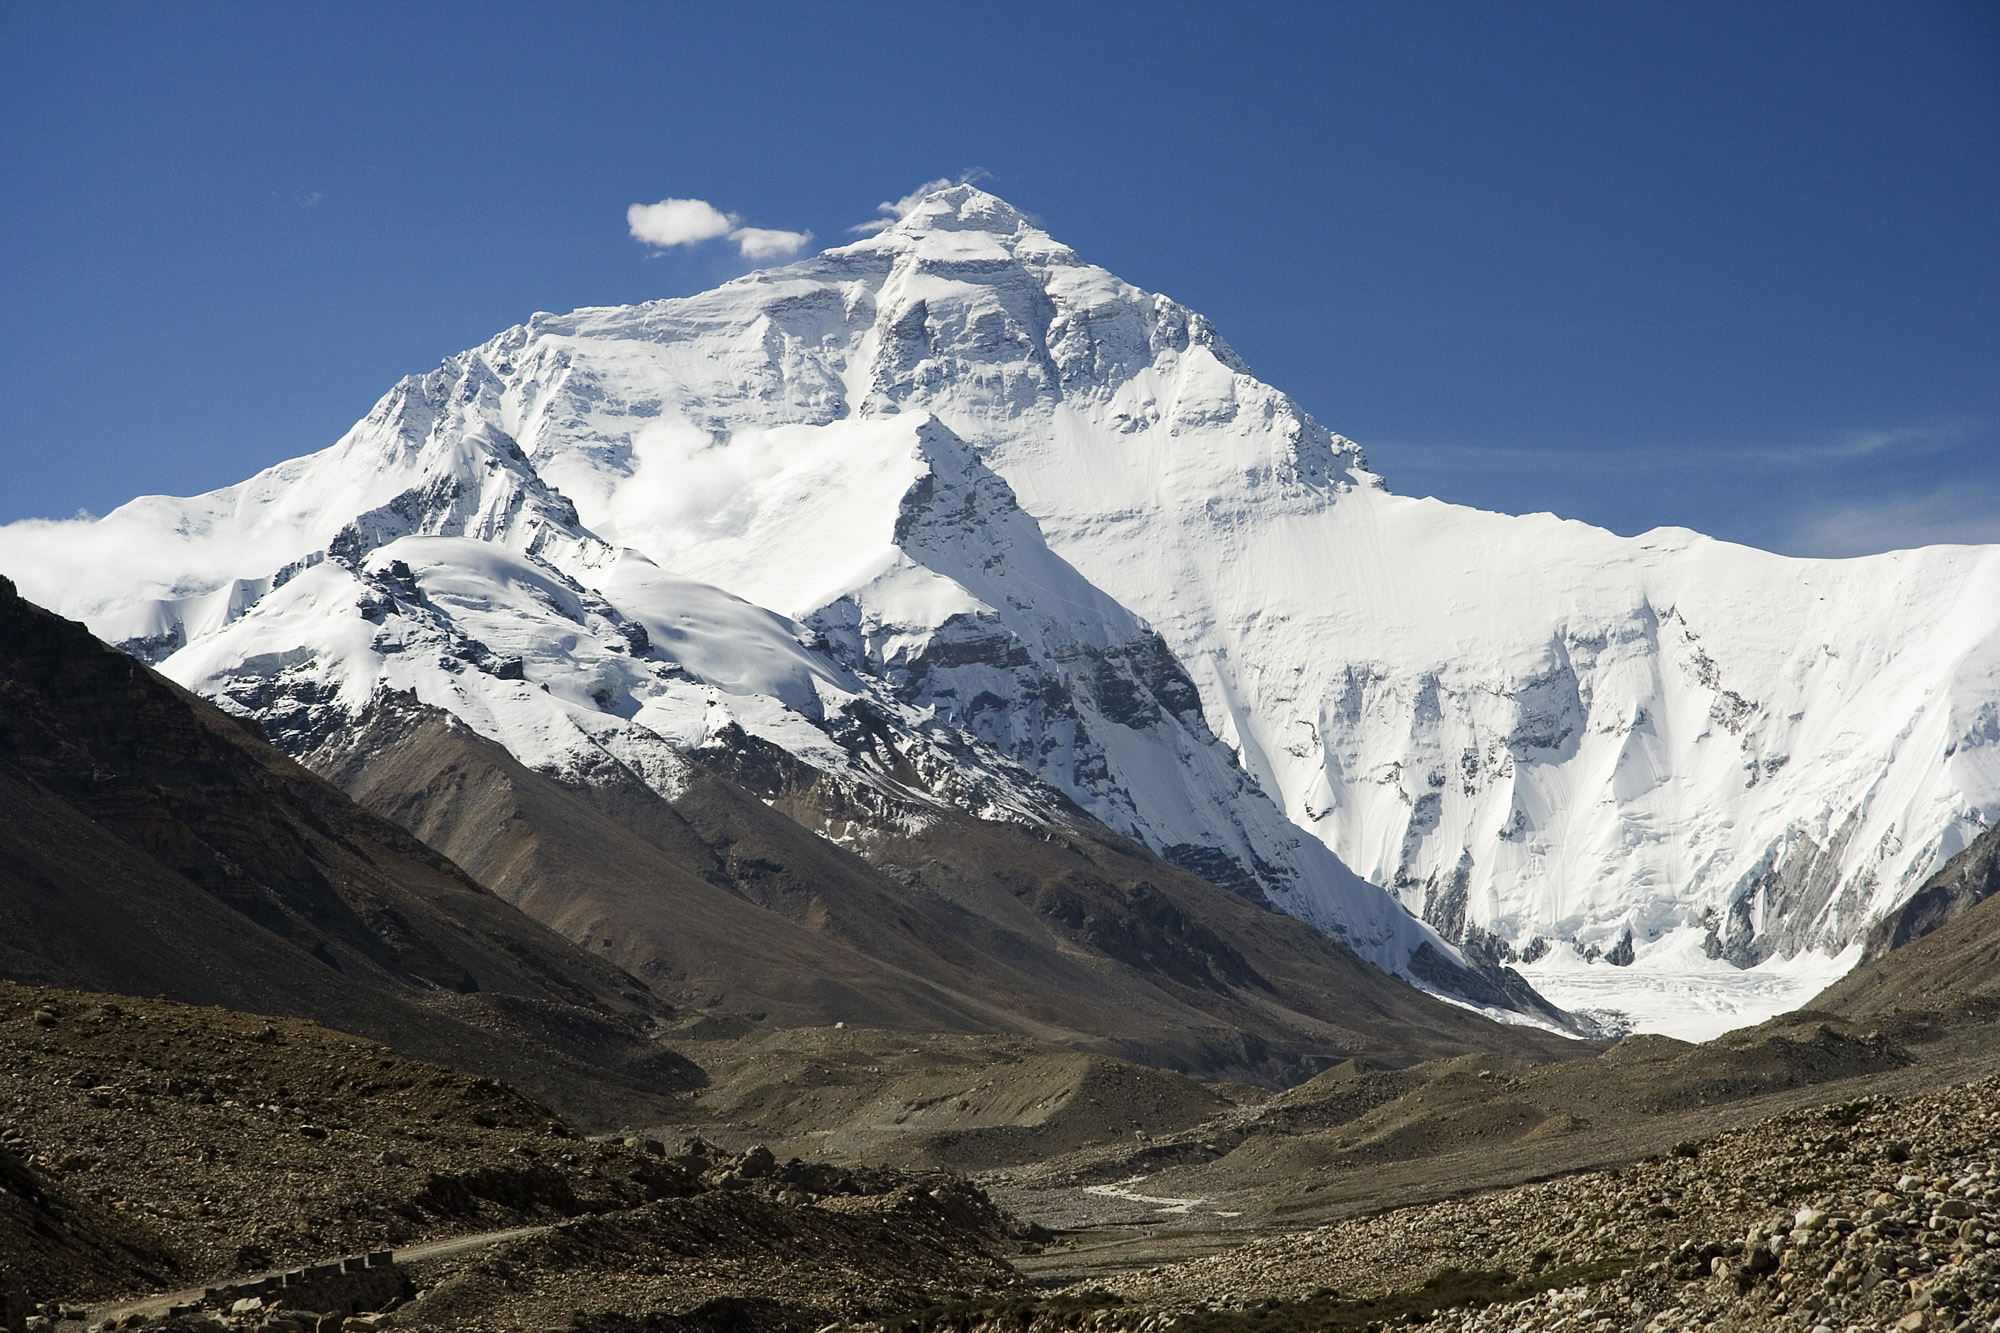
\includegraphics[width=0.99\textwidth]{everest.jpg}
    \caption{JPEG Downloaded from Internet}
    \label{fig:1}
\end{figure}
\subsubsection{Text}

\begin{figure}[H]
    \centering
    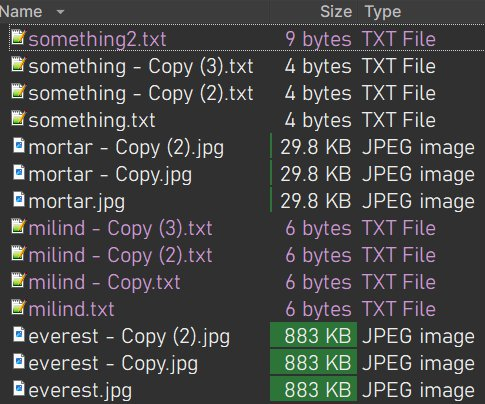
\includegraphics[width=0.99\textwidth]{things_made.jpg}
    \caption{Contents}
    \label{fig:1}

\end{figure}
\textbf{something.txt} was created and deleted. The file contained the following text:
\begin{verbatim}
test
\end{verbatim}
\noindent
\textbf{something.txt} was created and deleted. The file contained the following text:
\begin{verbatim}
test test
\end{verbatim}
This was done to check if the file was recoverable after deletion. The file was created using Notepad and saved in the logical partition.
\section{Imaging and Hash Verification}
\subsection{SHA256 Hash for something.txt}
\begin{verbatim}
    9f86d081884c7d659a2feaa0c55ad015a3bf4f1b2b0b822cd15d6c15b0f00a08
\end{verbatim}

\subsection{SHA256 Hash for something.txt after modifying}
\begin{verbatim}
    7e443c809e8ff0a43b9e53074098ffb5524be525e81b3bee0d37cf6ea9730011
\end{verbatim}

\subsection{SHA256 Hash for mortar.png}
\begin{verbatim}
    8c4345bda41f90d9693395383b99fcd14940c6629e4a218cb5a7cce6c0910fad
\end{verbatim}

\subsection{SHA256 Hash for everest.jpg}
\begin{verbatim}
    17912ca3fd92f220d331d80e799c1194c79ff2e7af453d05c261544c3bafecea
\end{verbatim}

\subsection{Hash Value Documentation}
\begin{itemize}
    \item The MD5 and SHA1 hashes were recorded at the time of image creation.
\end{itemize}
\begin{figure}[H]
    \centering
    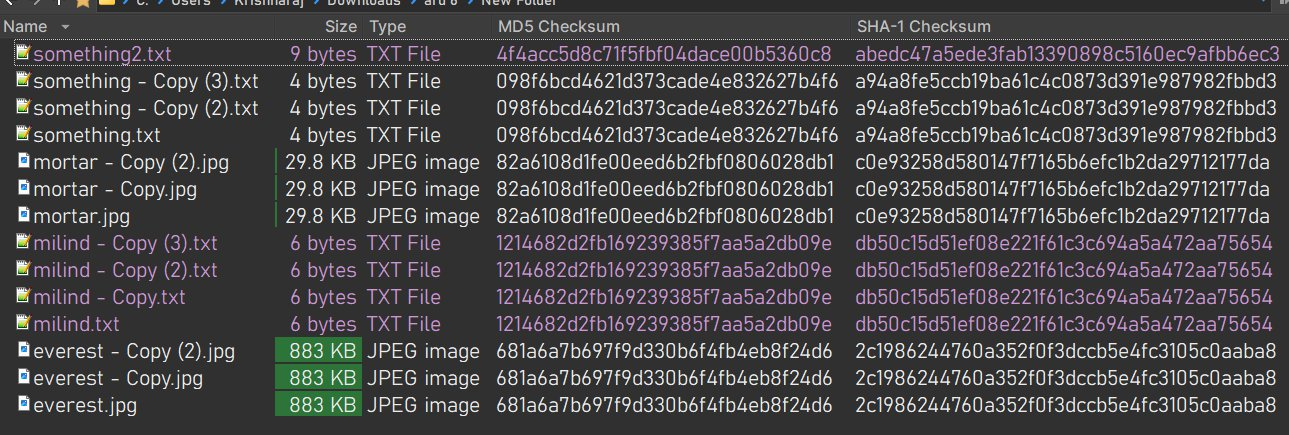
\includegraphics[width=0.99\textwidth]{checksums.jpg}
    \caption{}
    \label{fig:1}
\end{figure}

\section{Image Creation with FTK Imager}
\begin{itemize}
    \item The logical partition was imaged using FTK Imager Lite.
\end{itemize}
\begin{figure}[H]
    \centering
    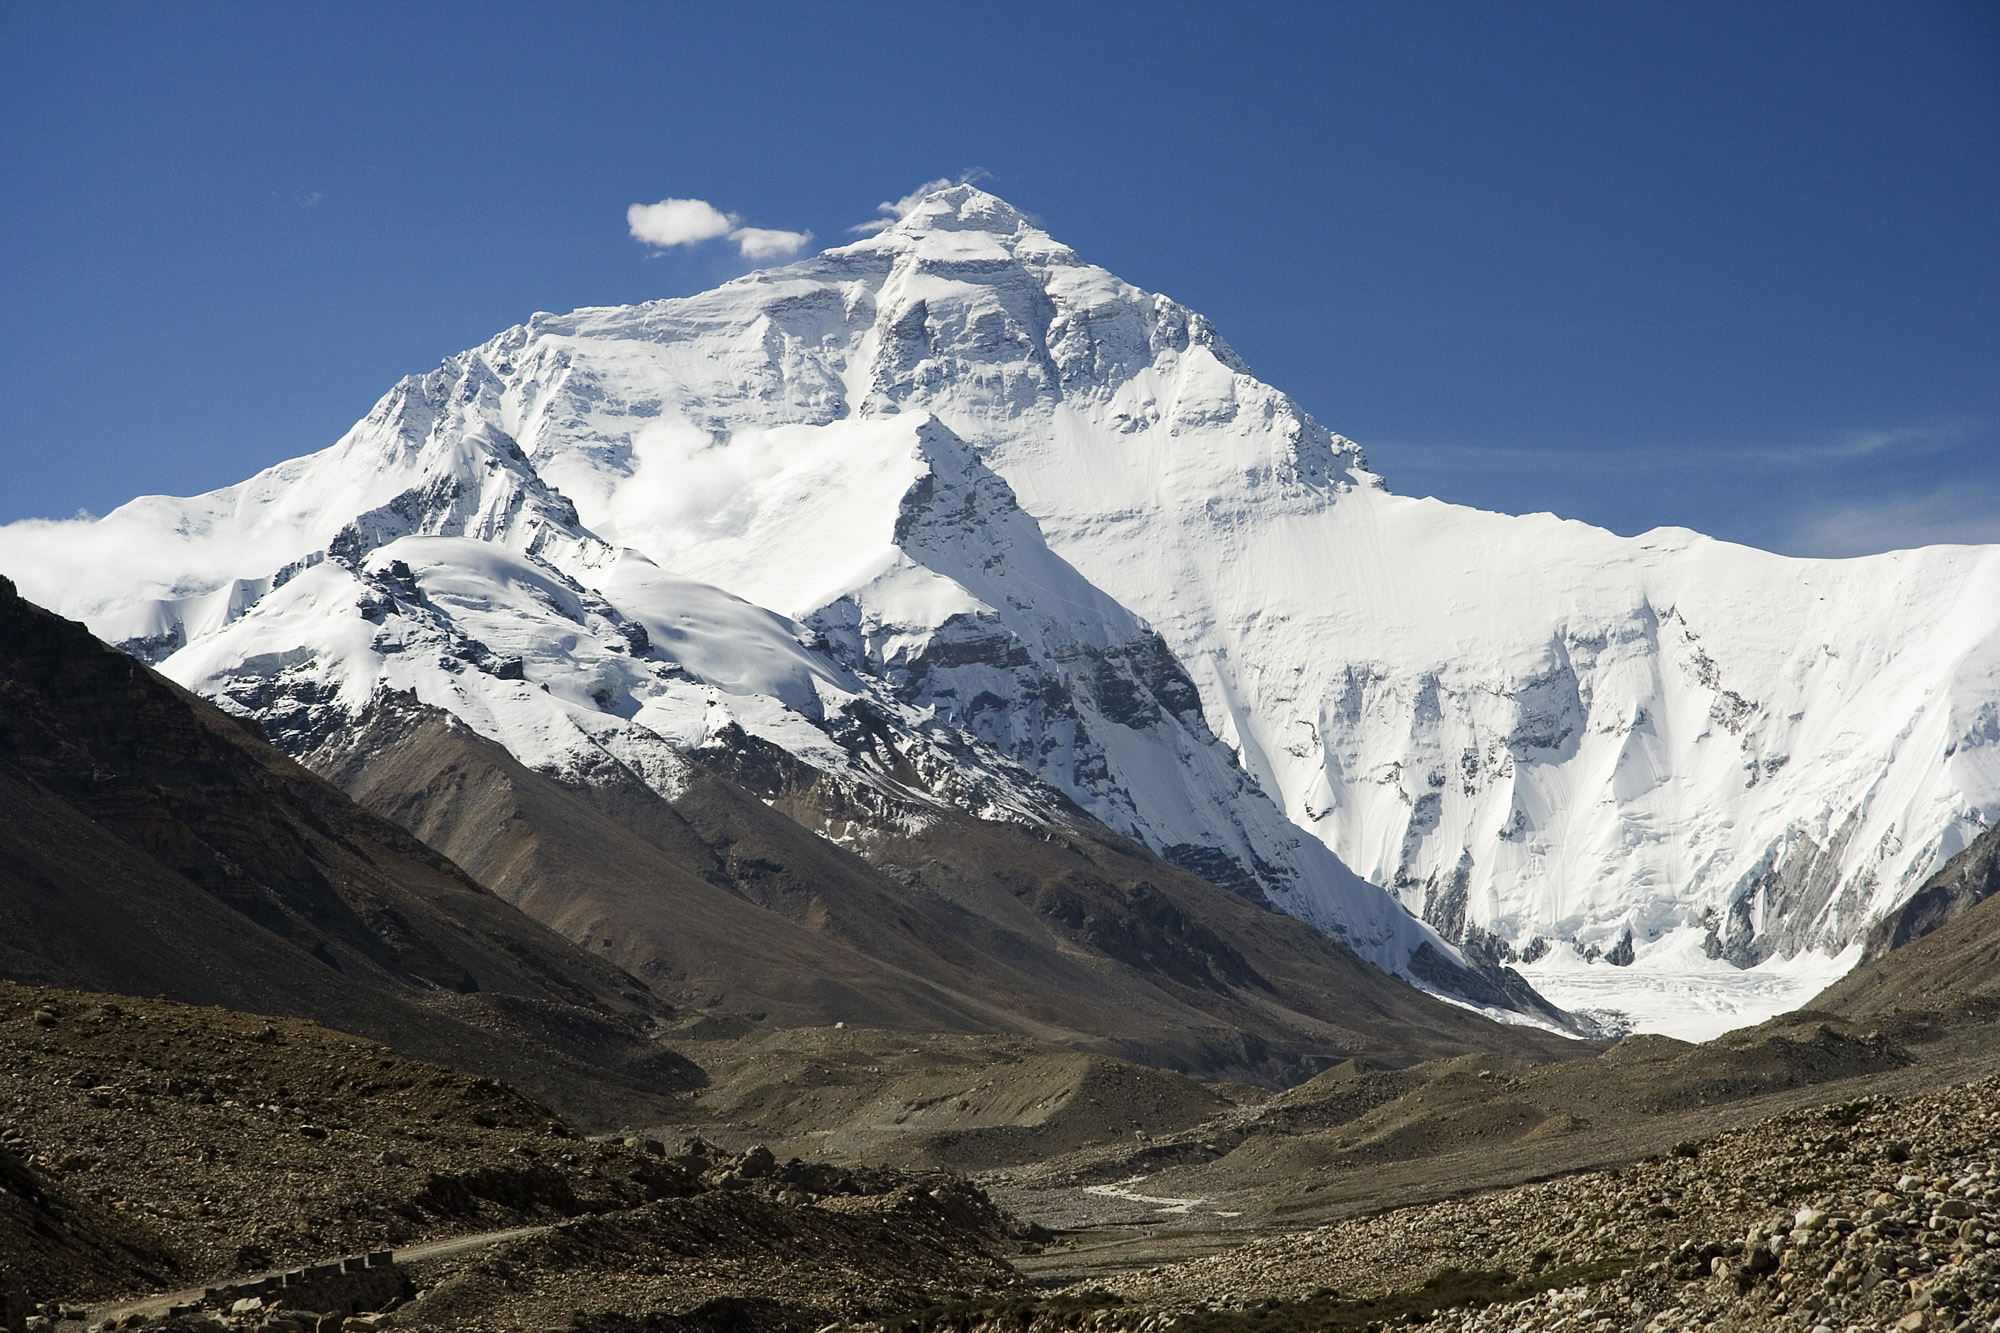
\includegraphics[width=0.99\textwidth]{everest.jpg}
    \caption{}
    \label{fig:1}
\end{figure}


\section{Analysis in Autopsy}

\subsection{Loading Image}
\begin{itemize}
    \item The forensic image was loaded into Autopsy for analysis.
\end{itemize}
\begin{figure}[H]
    \centering
    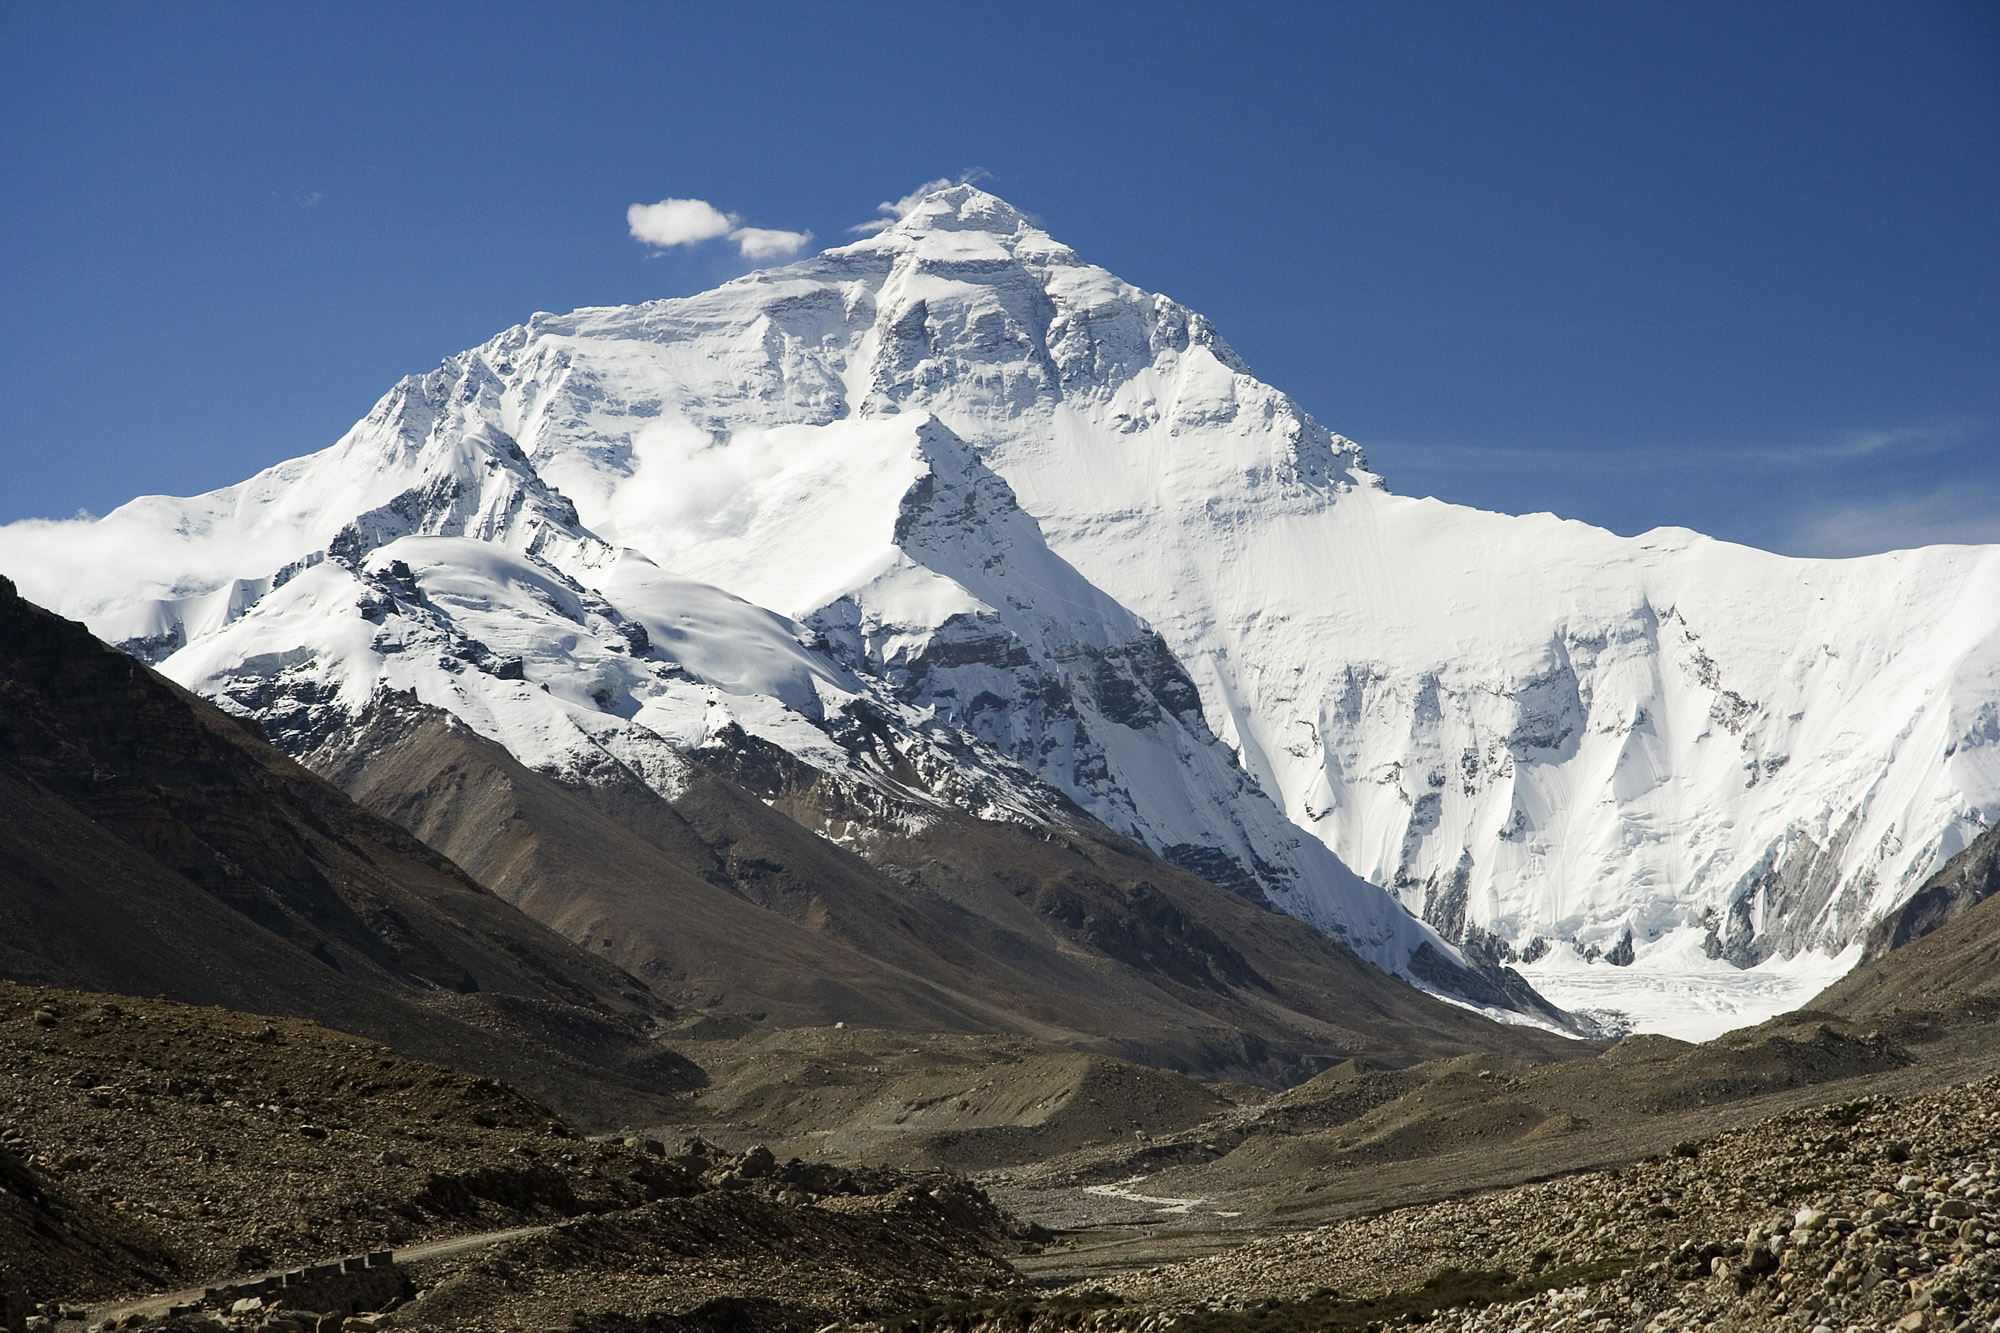
\includegraphics[width=0.99\textwidth]{everest.jpg}
    \caption{}
    \label{fig:1}
\end{figure}


\subsection{File Recovery Attempt}
\begin{itemize}
    \item Autopsy was used to attempt recovery of deleted files.
    \item The results varied based on the deletion scenario.
\end{itemize}
\begin{figure}[H]
    \centering
    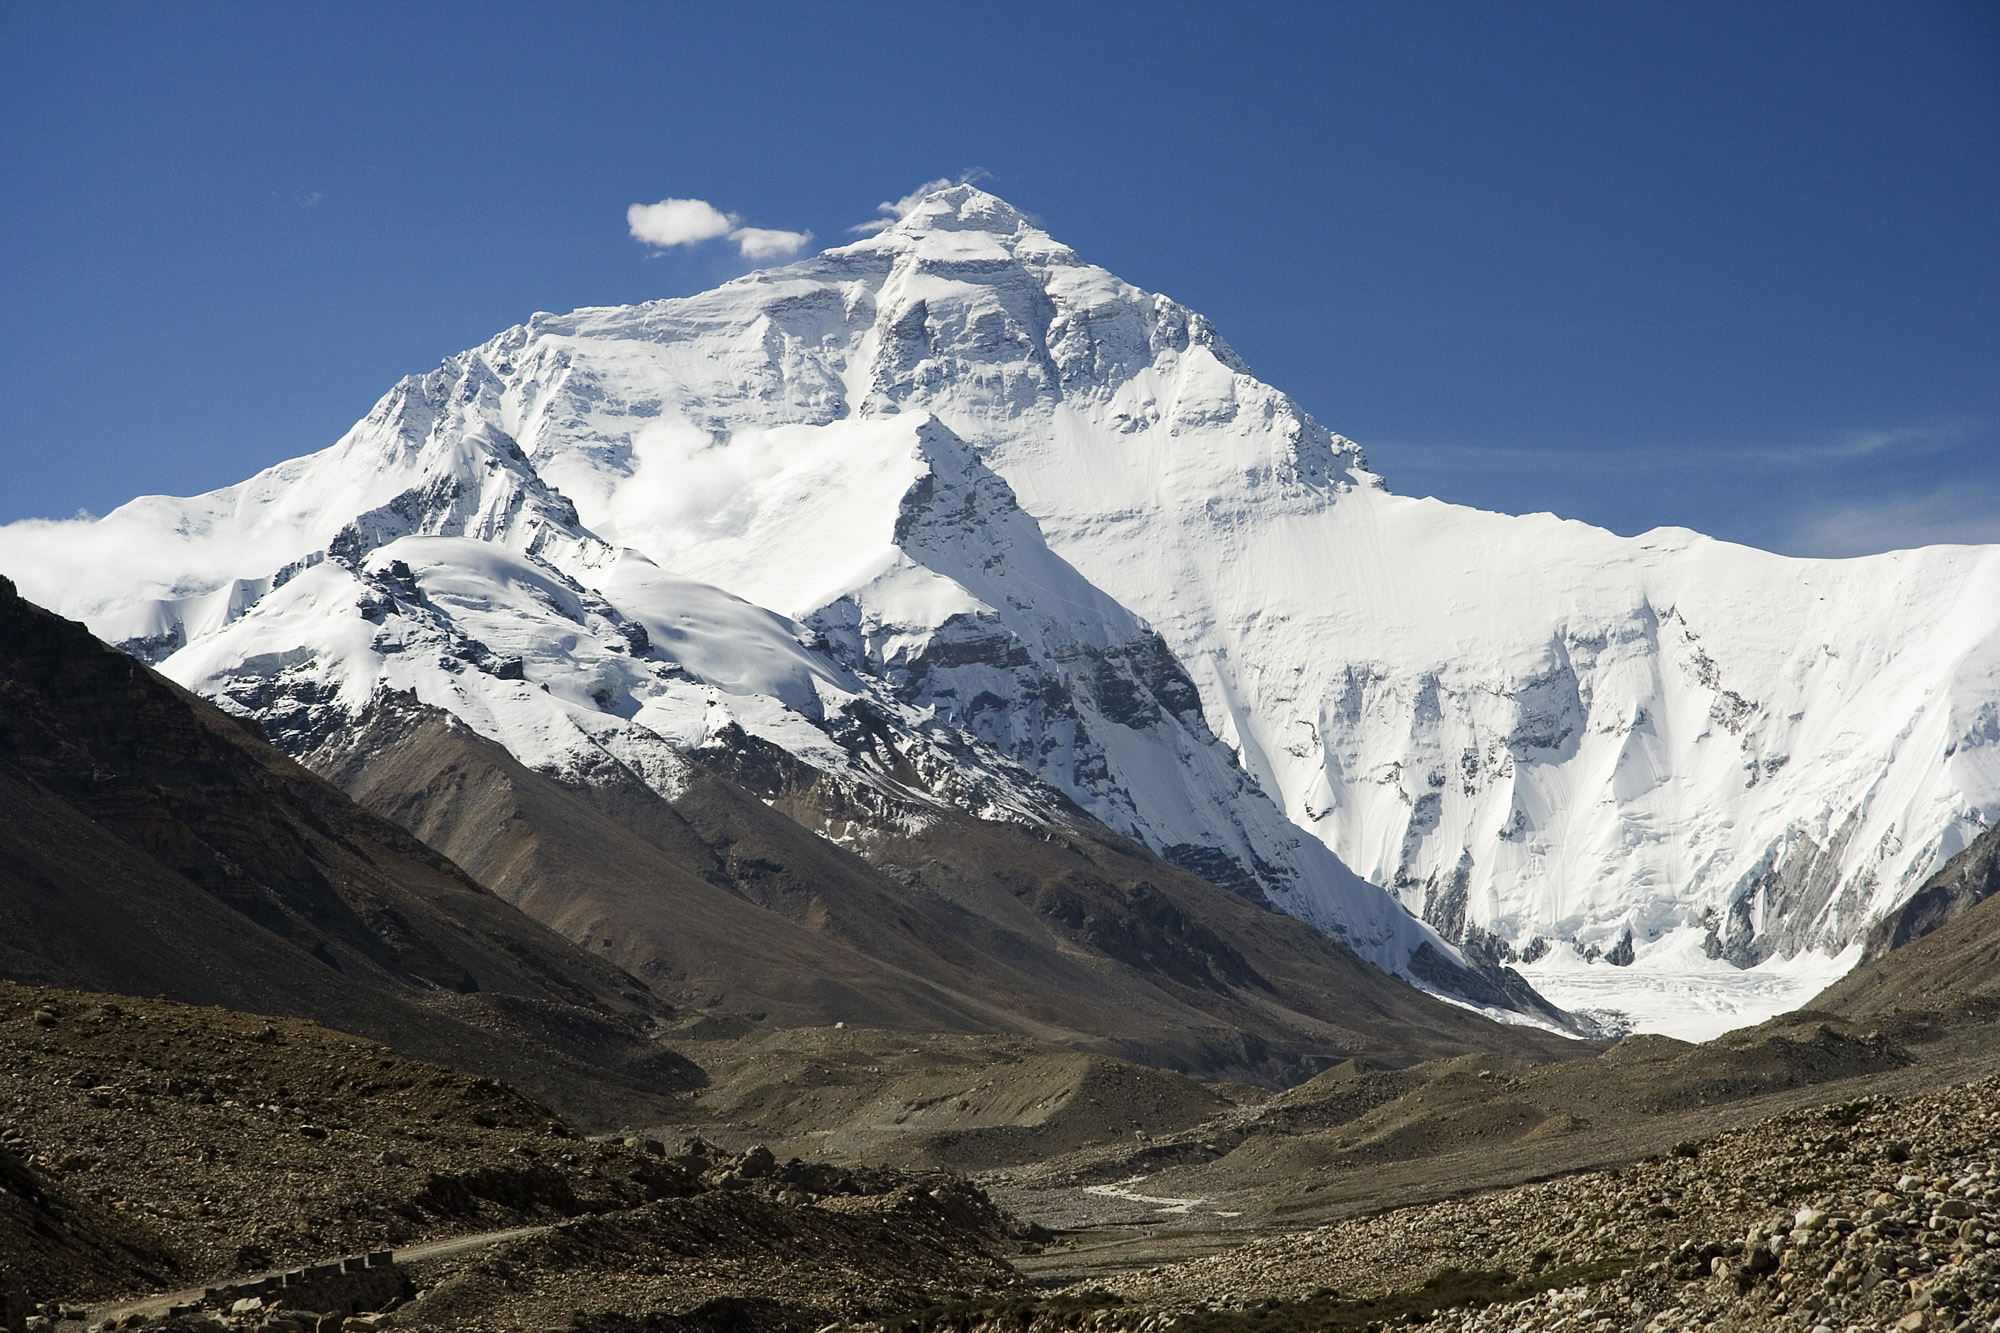
\includegraphics[width=0.99\textwidth]{everest.jpg}
    \caption{}
    \label{fig:1}
\end{figure}

\subsection{Autopsy Text Reports}

\begin{verbatim}
Created By Exterro® FTK® Imager 4.7.3.81 

Case Information: 
Acquired using: ADI4.7.3.81
Case Number: 1
Evidence Number: 11
Unique description: 1
Examiner: 1
Notes: 1

--------------------------------------------------------------

Information for C:\Users\Computer\Downloads\ard:

Physical Evidentiary Item (Source) Information:
[Device Info]
 Source Type: Logical
[Drive Geometry]
 Bytes per Sector: 512
 Sector Count: 38,912
[Physical Drive Information]
 Removable drive: False
 Source data size: 19 MB
 Sector count:    38912
[Computed Hashes]
 MD5 checksum:    9ea725c870a83043ea15b591d16abdd8
 SHA1 checksum:   2495b0f0da571ec75453f9000690528af61aefd6

Image Information:
 Acquisition started:   Tue Mar 25 09:49:46 2025
 Acquisition finished:  Tue Mar 25 09:49:47 2025
 Segment list:
  C:\Users\Computer\Downloads\ard.E01

\end{verbatim}


\section{Use Case Experiments and Results}

\subsection{Case 1: File Deleted and Removed from Trash}
\begin{itemize}
    \item The file was deleted and permanently removed.
    \item Recovery was possible using Autopsy.
\end{itemize}


\subsection{Case 2: File Deleted Using Erase Tools}
\begin{itemize}
    \item A secure delete tool (e.g., Eraser) was used.
    \item File recovery was not possible as data blocks were overwritten.
\end{itemize}


\subsection{Case 3: File Deleted and New File with Same Name Created}
\begin{itemize}
    \item The new file partially overwrote the original.
    \item Only the latest deleted file with the same name was recoverable.
\end{itemize}

\section{Conclusion}
\begin{itemize}
    \item FTK Imager Lite successfully captured forensic images and verified their integrity.
    \item Autopsy enabled effective analysis and partial recovery depending on the deletion method.
    \item Overwriting or secure deletion significantly reduced recovery success.
\end{itemize}

\clearpage
\begin{thebibliography}{99}
    \bibitem{ftk_imager}
    FTK Imager Lite. \\
    Website: \url{https://accessdata.com/products-services/ftk-imager-lite}

    \bibitem{autopsy}
    Autopsy. \\
    Website: \url{https://www.autopsy.com/}

    \bibitem{hashing}
    Hashing Algorithms (MD5, SHA1, SHA256). \\
    Website: \url{https://en.wikipedia.org/wiki/Cryptographic_hash_function}

    \bibitem{sleuth_kit}
    The Sleuth Kit (TSK). \\
    Website: \url{https://www.sleuthkit.org/}

    \bibitem{disk_management}
    Disk Management Utility (Windows). \\
    Website: \url{https://support.microsoft.com/en-us/windows/create-and-format-a-hard-disk-partition-in-windows}

    \bibitem{eraser_tool}
    Eraser - Secure Data Deletion Tool. \\
    Website: \url{https://eraser.heidi.ie/}
\end{thebibliography}

\end{document}